
%-------------------------------------------------------------------------------
%							SECOND SECTION
%-------------------------------------------------------------------------------

\section{Le transfert radiatif}


\begin{frame}
  \frametitle{Le phénomène du transfert radiatif}

  \scriptsize
Lorsque les photons se trouvent en présence de la matière, trois phénomènes majeurs (caractérisés par leurs opacités) se produisent :

\begin{columns}
  \begin{column}{0.55\textwidth}
    \scriptsize
   \begin{itemize}[<+>]
     \item \textbf{Émission} ($\sigma_e$) : des photons sont émis en réponse aux électrons excités descendants à des niveaux d’énergie plus bas. Plus la température matière est élevée, plus l'émission est importante % Typiquement on ne vas pas retrouver sigma_e dans nos equations car on va se placer dans l'ETL, et on Planck.
     \item \textbf{Absorption} ($\sigma_a$) : à l’inverse, certains photons sont absorbés, les électrons deviennent plus excités (ou se libèrent complètement de leurs atomes), et la matière se réchauffe. À l'équilibre thermique, $\sigma_a = \sigma_e$ % On va considerer en plus l'equilibre chimique ce qui donne l'ETL
     \item \textbf{Dispersion} ($\sigma_c$) : certains photons sont déviés de
     leur trajectoire originale par la matière. Il faut aussi tenir compte de la fonction de distribution angulaire de "scattering" $p(\bm{\Omega^\prime \rightarrow \bm{\Omega}})$ \parencite{Reference3}.
   \end{itemize}
  \end{column}
  % \pause
  \begin{column}{0.45\textwidth}
     \begin{figure}       
      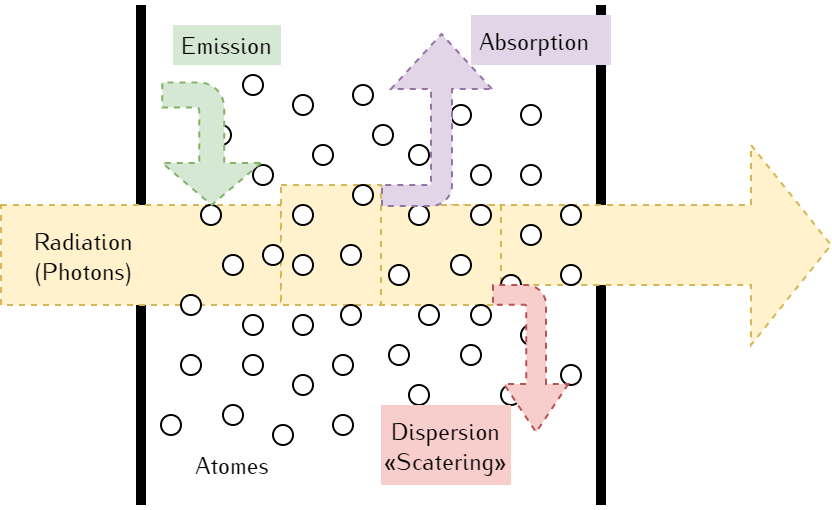
\includegraphics[width=5cm]{TransferRadiatif}       
      \caption{Interaction entre matière et radiation}
    \end{figure}
  \end{column}
 \end{columns}
 
\end{frame}

\begin{frame}
  \frametitle{L'ETR}
  L'équation du transfert radiatif (ETR) est un bilan d'énergie lié au rayonnement au niveau mésoscopique (dans la direction $\bm{\Omega}$). 

  \begingroup
  \scriptsize
  \begin{gather*}
      \begin{aligned}
        \alert<1>{\frac{1}{c} \frac{\partial}{\partial t}I(t,\bvec{x},\bm{\Omega},\nu)} &\alert<1>{+\bm{\Omega}\cdot\nabla_{\bvec{x}} I(t,\bvec{x},\bm{\Omega},\nu)} \\
      &\alert<2>{= \sigma_a(\rho,\bm{\Omega},\nu)\left(B(\nu,T)-I(t,\bvec{x},\bm{\Omega},\nu)\right)} \\
      &\alert<3>{+ \frac{1}{4\pi} \int_{0}^{\infty} \int_{S^2}\sigma_c(\rho,\bm{\Omega},\nu)p(\bm{\Omega}^\prime\rightarrow\bm{\Omega})\left(I(t,\bvec{x},\bm{\Omega}^\prime,\nu)-I(t,\bvec{x},\bm{\Omega},\nu)\right) \, d\bm{\Omega}^\prime \, d\nu}
      \end{aligned}
  % \label{eqn:ETR}
  \end{gather*}
  \endgroup
où :
\begin{itemize}
  \item $I(t,\bvec{x},\bm{\Omega},\nu)$ désigne l'intensité radiative spécifique
  \item $B(\nu,T)$ la fonction de Planck, caractérise l'émission à l'ETL
  \item $\oint p(\bm{\Omega}^\prime\rightarrow\bm{\Omega})\, d\bm{\Omega}^\prime=1$
\end{itemize}

\end{frame}

\begin{frame}
  \frametitle{Le modèle P1}
%   \footnotesize
  Le modèle P1 donne une simplification de l'ETR en vue des simulations. %Le terme 1/3
  \begingroup
  \footnotesize
  \begin{equation*}
      \begin{cases}
        \alert<1->{\partial_tE + c \operatorname {div} \bvec F = c\sigma_a\left(aT^4-E\right)}\\
        \alert<1->{\partial_t\bvec{F} + c \nabla E = -c\sigma_c \bvec{F}} \\
        \alert<1->{\rho C_v \partial_t T = c \sigma_a \left(E-aT^4\right)}
      \end{cases}
  % \label{eqn:P1}
  \end{equation*}
  \endgroup
  où :   % Moins precis que Monte-Carlo ou ordonne discretes; Mais plus rapide et suddisant; sigma
\begin{itemize}
  \item Energie des photons : $E(t,\bvec{x}) = \frac{4\pi}{c} \int_{0}^{\infty} \int_{S^2} I(t,\bvec{x},\bm{\Omega},\nu) \, d\bm{\Omega} \, d\nu$
  \item Flux des photons :    $\bvec{F}(t,\bvec{x}) = \frac{4\pi}{c} \int_{0}^{\infty} \int_{S^2} \bm{\Omega}I(t,\bvec{x},\bm{\Omega},\nu) \, d\bm{\Omega} \, d\nu$  
  % \label{eqn:EFT}
\end{itemize}
\pause
% \normalsize
Ce modèle est :
\begin{itemize}[<+>]
  \item Linéaire et hyperbolique
  \item Macroscopique aux moments (d’ordre 2), dit "gris"
  \item Moins précis qu'un modèle résolut par la méthode de Monte-Carlo 
  \item Peu coûteux et rapide à implémenter
\end{itemize}

\end{frame}

\setbeamercovered{invisible}

\begin{frame}
  \frametitle{Le schéma de "splitting"}
  Le principe :
  \footnotesize
  \begin{enumerate}
    \item<1-> On sépare le problème en temps en deux
    \item<2-> On résout l'étape 1 (réglage de la température) : sur une maille, schéma d'Euler implicite et méthode du point fixe
    $$     \begin{cases}
      \partial_tE + \alert{\underbrace{c \operatorname {div} \bvec F}_{=\,0}} = c\sigma_a\left(aT^4-E\right)\\
      \rho C_v \partial_t T = c \sigma_a \left(E-aT^4\right) 
     \end{cases} $$
    \item<3-> On résout l'étape 2 (partie hyperbolique) : volume finis 2D
    $$     \begin{cases}
      \only<3->{\partial_tE + c \operatorname {div} \bvec F = \alert{\underbrace{c\sigma_a\left(aT^4-E\right)}_{=\,0}}}\\
      \only<3->{\partial_t\bvec{F} + c \ \nabla E = -c\sigma_c \bvec{F}} \\
     \end{cases} $$
    \item<4> \alert {Tout ceci se fait sur le meme pas de temps!}
  \end{enumerate}

\end{frame}
\setbeamercovered{transparent}


\begin{frame}
  \frametitle{Le schéma de "splitting" : Étape 1}
  % Reglage de la temperature 
  \begin{columns}
    \begin{column}{0.5\textwidth}
     À l'itération $n$, on pose $\Theta = aT^4$

      \begingroup
      \normalsize
      \begin{equation*} 
        \begin{dcases}
         \alert<1->{E_j^{q+1} = \dfrac{\alpha E_j^n + \beta \gamma \Theta_j^n}{1 - \beta \delta}} \\
         \alert<1->{\Theta_j^{q+1} = \dfrac{\gamma \Theta_j^n + \alpha \delta E_j^n}{1 - \beta \delta}}
        \end{dcases}
    \label{eqn:Step1}
    \end{equation*}
      \endgroup
      Où
      \tiny
      $\mu_q = \dfrac{1}{T^{3,n} + T^{n}T^{2,q} + T^{q}T^{2,n} + T^{3,q}}$
      \normalsize
    \end{column}
    % \pause
    \begin{column}{0.5\textwidth}
       \begin{center}
        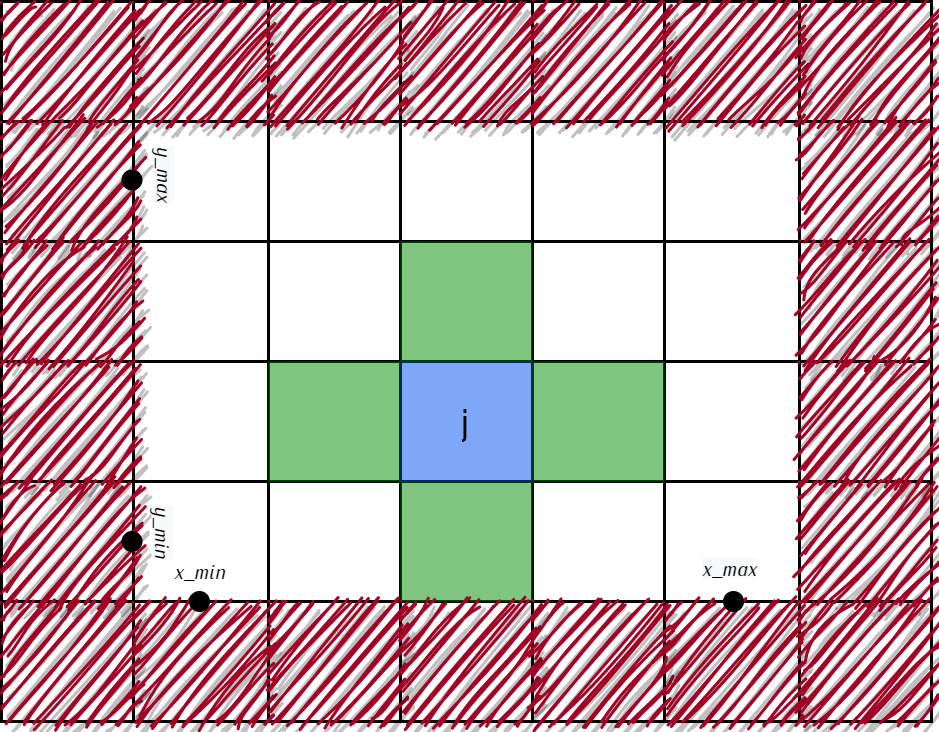
\includegraphics[width=4.5cm]{Dicretisation2D}       
       \end{center}
    \end{column}
   \end{columns}
   \tiny
  $\quad  \alpha = \dfrac{1}{\Delta t \left( \frac{1}{\Delta t} + c \sigma_a \right)} ,\quad 
   \beta = \dfrac{c \sigma_a}{\frac{1}{\Delta t} + c \sigma_a} ,\quad 
   \gamma = \dfrac{\rho_j C_v \mu_q}{\Delta t \left( \frac{\rho_j C_v \mu_q}{\Delta t} + c \sigma_a \right)} \quad , \quad  
   \delta = \dfrac{c \sigma_a}{\frac{\rho_j C_v \mu_q}{\Delta t} + c \sigma_a}.$

   \normalsize
   \begin{columns}
    \begin{column}{1.0\textwidth} 
      \\
      Itération sur $q$ ; convergence vers $E_j^*$ et $\Theta_j^*$ ; $\bvec F_j = \bvec F_j^*$ constant.
    \end{column}
    \begin{column}{0.0\textwidth} 
    \end{column}
  \end{columns}
   
\end{frame}


\begin{frame}
  \frametitle{Le schéma de "splitting" : Étape 2}   % Adaptable aussi en 2D
  \begin{columns}
    \begin{column}{0.6\textwidth}
      \begingroup
      \normalsize
      \begin{equation*} 
          \begin{dcases}
          \alert<1->{E_j^{n+1} = E_j^* + \alpha \sum_k \left( \bvec F_{jk}, \bvec n_{jk} \right)} \\
          \alert<1->{\bvec{F}_j^{n+1} = \beta \bvec F_j^* + \bm{\gamma} E_j^n + \delta \sum_k E_{jk} \bvec n_{jk}}
          \end{dcases}   
      % \label{eqn:Step2}
      \end{equation*}
      Avec :
      \newline
      % \begingroup
      \scriptsize
    
      % \begin{gather*}    
      % \begin{aligned} 
        $\alpha = -\frac{c \Delta t}{\left| \Omega_j \right|}, \linebreak
        \beta = \frac{1}{\Delta t} \left( \frac{1}{\Delta t} + c \sum_k M_{jk} \sigma_{jk} \right)^{-1}, \linebreak
        \bm{\gamma} = \frac{c}{\left| \Omega_j \right|} \left( \frac{1}{\Delta t} + c \sum_k M_{jk} \sigma_{jk} \right)^{-1} \left( \sum_k l_{jk} M_{jk} \bvec n_{jk} \right) \linebreak
        \delta = -\frac{c}{\left| \Omega_j \right|} \left( \frac{1}{\Delta t} + c \sum_k M_{jk} \sigma_{jk} \right)^{-1}$
    %   \end{aligned}
    % \end{gather*}

    \endgroup
      
    \end{column}
    % \pause
    \begin{column}{0.4\textwidth}
      % \begin{figure}
      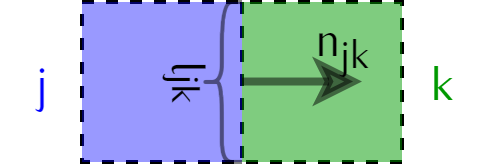
\includegraphics[width=5cm]{Interaction2D}       
        % \caption{Interaction entre deux mailles}
      % \end{figure}
       \begin{center}
        \begingroup
        \tiny
        \begin{align*}
          \left(\bvec F_{jk}, \bvec n_{jk} \right) &= l_{jk} M_{jk} \left( \frac{\bvec F_j^n \cdot \bvec n_{jk} + \bvec F_k^n \cdot \bvec n_{jk}}{2} - \frac{E_k^n - E_j^n}{2} \right) \\
          E_{jk} \bvec n_{jk} &= l_{jk} M_{jk} \left( \frac{E_j^n + E_k^n}{2} - \frac{\bvec F_k^n \cdot \bvec n_{jk} - \bvec F_j^n \cdot \bvec n_{jk}}{2} \right) \bvec n_{jk} \\
        %  \end{align*}
        %  \begin{align*}
          M_{jk} &= \frac{2}{2 + \Delta x \sigma_{jk}}  \\
          \sigma_{jk} &= \frac{1}{2} \left( \sigma_c(\rho_j,T_j^n) + \sigma_c(\rho_k,T_k^n) \right)
         \end{align*}
        \endgroup
       \end{center}
    \end{column}
   \end{columns}
\end{frame}

\begin{frame}
  \frametitle{Implémentation C++}
  \begin{columns}
    \begin{column}{0.5\textwidth}
      \scriptsize
      \begin{itemize}
        \item Temps final = 0.01 \si{sh} %\textit{(1 shake (\si{sh}) = $10^{-8}$ secondes)}
        \item $c = 299$ [\si{\cm \per sh}]
        \item $a = 0.01372$ [\si{g \per cm \per sh^2  \per keV }]
        \item $C_v = 0.14361$ [\si{Jerk \per\g \per keV}] % \textit{(1 \si{Jerk} = 1\si{m \per \s\cubed})}
        \item La densité $\rho$ est un signal complet [\si{\g\per\cm\cubed}]
        \item $\sigma_a = \rho T$ [\si{\per\cm}]
        \item $\sigma_c = \rho T$ [\si{\per\cm}]
        \item $T_0, T_{gauche} = 5$ [\si{keV}] % \textit{(en termes de température, 1 \si{keV} = 11605 \si{K})}
        \item $E_0 = aT_0^4$ [\si{g \per \cm \per sh^2}]
        \item $E_{gauche^*} = aT_{0}^4 + 5 \sin (2 k \pi t)$ [\si{g \per \cm \per sh^2}]
        \item $\bvec{F}_0, \bvec{F}_{gauche} = \bvec{0}$ [\si{g \per sh^2}]
        \item Sorties libres sur les autres bords
      \end{itemize}
    \end{column}


    \begin{column}{0.5\textwidth}
       \begin{figure}
        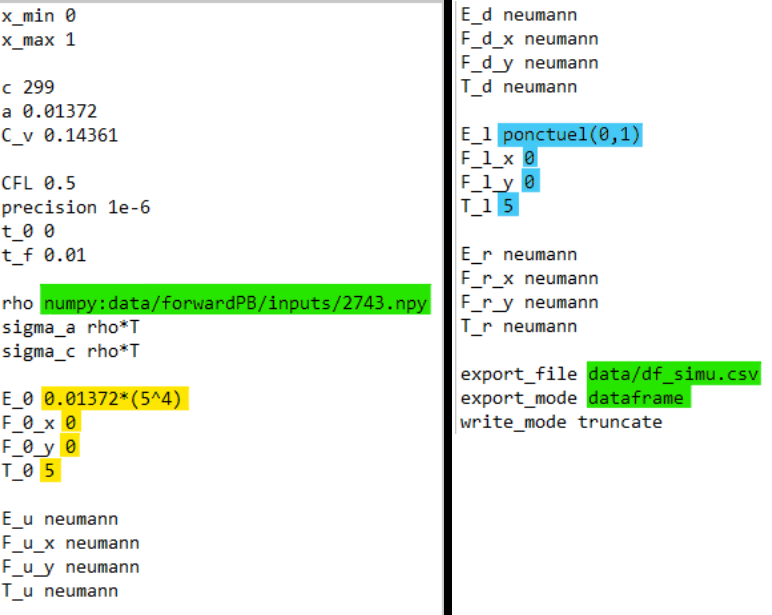
\includegraphics[width=5cm]{SimuCFG}   % EN 2D    
        \only{\caption{Exemple de fichier configuration}}
      \end{figure}
    \end{column}
   \end{columns}

\end{frame}
